\section{Besonderes elektronisches Anwaltspostfach}
Das Gesetz zur Förderung des elektronischen Rechtsverkehrs mit den Gerichten hatte die Modernisierung der Kommunikation mit der Justiz vorgeschrieben. ''[...] Damit soll zugleich der derzeit noch bestehende ''Flickenteppich'' beim elektronischen Rechtsverkehr innerhalb der einzelnen Bundesländer beseitigt und eine bundesweit flächendeckende elektronische Infrastruktur geschaffen werden. Das beA wird – ggf. nach einer kurzen Umstellungsphase – zu einer Effektivierung und Beschleunigung der Arbeitsabläufe innerhalb der Kanzlei führen. Mittelfristig wird die ausschließlich elektronische Kommunikation zu einer Verkürzung der Postlaufzeiten und einer Einsparung an Druck-, Papier- und Portokosten führen. [...]'' \textcite{bea:bea:praxis:qa}\footfullcite{bea:bea:praxis:qa} \\
Infolgedessen wurde durch die Neuregelung in der Zivilprozessordnung (kurz ZPO) und in anderen Verfahrensordnungen die elektronischen Zugangswege für die Anwaltschaft zur Justiz erweitert. Lediglich die Verfassungs- und die Strafgerichtsbarkeit bleiben ausgenommen. Dadurch wurde auch auf die geringe Akzeptanz und Verbreitung des bisher (un)genutzten EGVPs und auf die hohen Sicherheitsmängel von dessen Nachfolger, der De-Mail, reagiert. \\
Gemäß §31a der Bundesrechtsanwaltsordnung (kurz BRAO) ist die Bundesrechtsanwaltskammer (kurz BRAK) verpflichtet zum 01.01.2016 jedem zugelassenen Rechtsanwalt ein besonderes elektronisches Anwaltspostfach (kurz beA) einzurichten. Fortan soll jede elektronische Kommunikation von Anwälten untereinander und zu den Gerichten ausschließlich über dieses Postfach stattfinden. Damit löst das beA das bisher genutzte EGVP für Rechtsanwälte ab.

\subsection{Rechtliche Rahmenbedingungen}
Im Vorfeld wurde heftig über die rechtlichen Rahmenbedingungen diskutiert. Man wolle den elektronischen Rechtsverkehr \textit{fördern}. So solle festgelegt werden, dass es eine verbindliche Verpflichtung zur Benutzung des beA für Rechtswälte gibt. Allerdings sollten auch einige Gesetze entschärft werden. So plädierte man auf die Absenkung des extrem hohen Signaturniveaus und auf die Zulassung anderer sicherer Standards, wie zum Beispiel die organisationsbezogene elektronische Signatur. Weiterhin sollte den Ländern Zeit gewährt werden, um den elektronischen Rechtsverkehr (kurz ERV) flächendeckend und stufenweise einzuführen. Weitere Forderungen der BRAK - wie zum Beispiel der Verzicht auf Zustellungsnachweise von Anwälten, die Ersetzung von Papierbekanntmachungen und -veröffentlichungen durch Internetveröffentlichungen und die vorbehaltlose Zulassung unterschriftsloser gerichtlicher Dokumente, die auf Druckstraßen erstellt wurden, sind beim Gesetzgeber eingereicht worden. \\
Mit der Veröffentlichung der Artikel §31, §31a und §31b BRAO wurden die generellen Anforderungen an das besondere elektronische Anwaltspostfach gesetzlich festgehalten. Darin ist zusammengefasst folgendes festgehalten:
\begin{itemize}
	\item Die BRAK ist dazu verpflichtet zum 01.01.2016 jedem zugelassenen Rechtsanwalt ein besonderes elektronisches Anwaltspostfach (kurz beA) einzurichten. Dazu wird es ein Verzeichnis geben, dass alle zugelassenen Rechtsanwälte enthält und vom Bundesministerium der Justiz geführt und gepflegt wird.
	\item Die BRAK stellt sicher, dass der Zugang zum beA durch ein sicheres Verfahren mit zwei voneinander unabhängigen Sicherungsmittel möglich ist.
	\item Mit dem Verlust der Zulassung erlischt auch die Zugangsberechtigung zum beA. Das Postfach des Anwalts wird außerdem gelöscht.
\end{itemize}

Um das besondere elektronische Anwaltspostfach sicher zu gestalten, sollten die typischen sicherheitstechnischen Aspekte beachtet werden. Vor allem die Authentizität einer Person im System und die Integrität einer jeden Nachricht müssen gewährleistet werden. Weitere wichtige Aspekt sind der Datenschutz der gesicherten Nachrichten und Dokumente im Postfach und das elektronische Empfangsbekenntnis, welches besonders bei der Einhaltung von Fristen bedeutsam ist. Genaue Details sind in der Zivilprozessordnung §130a festgehalten:

\begin{quote}
	\begin{center}
		\textbf{§ 130a} \\
		\textbf{Elektronisches Dokument}
	\end{center}
	(1) Soweit für vorbereitende Schriftsätze und deren Anlagen, für Anträge und Erklärungen der Parteien sowie für Auskünfte, Aussagen, Gutachten und Erklärungen Dritter die Schriftform vorgesehen ist, genügt dieser Form die Aufzeichnung als elektronisches Dokument, wenn dieses für die Bearbeitung durch das Gericht geeignet ist. Die verantwortende Person soll das Dokument mit einer qualifizierten elektronischen Signatur nach dem Signaturgesetz versehen. Ist ein übermitteltes elektronisches Dokument für das Gericht zur Bearbeitung nicht geeignet, ist dies dem Absender unter Angabe der geltenden technischen Rahmenbedingungen unverzüglich mitzuteilen. \\
	(2) Die Bundesregierung und die Landesregierungen bestimmen für ihren Bereich durch Rechtsverordnung den Zeitpunkt, von dem an elektronische Dokumente bei den Gerichten eingereicht werden können, sowie die für die Bearbeitung der Dokumente geeignete Form. Die Landesregierungen können die Ermächtigung durch Rechtsverordnung auf die Landesjustizverwaltungen übertragen. Die Zulassung der elektronischen Form kann auf einzelne Gerichte oder Verfahren beschränkt werden. \\
	(3) Ein elektronisches Dokument ist eingereicht, sobald die für den Empfang bestimmte Einrichtung des Gerichts es aufgezeichnet hat.
\end{quote}

Ein weiteres wichtiges Merkmal stellt hier die qualifizierte elektronische Signatur (qeS) dar. Sie wird benutzt, um eine elektronische Nachricht oder ein elektronisches Dokument zu signieren, somit elektronisch zu unterschreiben, sodass anhand der Signatur der Urheber der Nachricht eindeutig ermittelt werden kann. Dies erfüllt den Anspruch nach Authentizität. \\
Gemäß § 130a ZPO-neu können ab 2018 elektronische Dokumente entweder qualifiziert elektronisch signiert oder über einen anderen ''sicheren Übermittlungsweg'' bei Gericht eingereicht werden, wie zum beispielsweise über das besondere elektronische Anwaltspostfach. Voraussetzung für den Verzicht auf die qeS ist allerdings ein sicheres Anmeldeverfahren vor dem Versand.
\\
Laut ZPO §130d wird die bereits zuvor angesprochene Nutzungspflicht für Rechtsanwälte und Behörden gesetzlich festgeschrieben. Dadurch müssen diese Parteien das beA benutzen und können bei Verweigerung sogar rechtlich belangt werden. Diese Regelung tritt für Rechtsanwälte und Behörden mit dem 01.01.2016 (spätestens mit dem 01.01.2022) in Kraft.

\begin{quote}
	\begin{center}
		\textbf{§ 130d} \\
		\textbf{Nutzungspflicht für Rechtsanwälte und Behörden}
	\end{center}
	Vorbereitende Schriftsätze und deren Anlagen sowie schriftlich einzureichende Anträge und Erklärungen, die durch einen Rechtsanwalt, durch eine Behörde oder durch eine juristische Person des öffentlichen Rechts einschließlich der von ihr zur Erfüllung ihrer öffentlichen Aufgaben gebildeten Zusammenschlüsse eingereicht werden, sind als elektronisches Dokument zu übermitteln. Ist dies aus technischen Gründen vorübergehend nicht möglich, bleibt die Übermittlung nach den allgemeinen Vorschriften zulässig. Die vorübergehende Unmöglichkeit ist bei der Ersatzeinreichung oder unverzüglich danach glaubhaft zu machen; auf Anforderung ist ein elektronisches Dokument nachzureichen.
\end{quote}

Allerdings wird keine Nutzungspflicht für Gerichte in §130d ZPO beschrieben. Für die Justiz gibt es derzeit keine entsprechende gesetzliche Verpflichtung. Den Ländern soll zunächst die Möglichkeit gegeben werden, für die betroffenen Gerichtsbarkeiten/Gerichtszweige die notwendigen Infrastrukturen und technischen Ausstattungen zu schaffen.

\subsection{Zeitplan}
Der folgende Zeitplan ist aus dem BRAKMagazin 2/2015, April 2015\textcite{bea:bea:brak2/2015} entnommen.
\begin{itemize}
\item \textbf{2016:} Am 1.1.2016 wird das beA-System mit etwa 165.000 Anwaltspostfächern in Betrieb genommen. So sieht es das Gesetz zur Förderung des elektronischen Rechtsverkehrs mit den Gerichten (ERV-Gesetz) vor. [...]
\item \textbf{2018:} Ab 2018 sollen alle Gerichte der Zivil-, Arbeits-, Finanz-, Verwaltungs- und Sozialgerichtsbarkeit für die elektronische Kommunikation über das beA erreichbar sein. Allerdings besteht für die Länder die Möglichkeit, diesen Zeitpunkt um ein oder zwei Jahre nach hinten zu verschieben.
\item Ab \textbf{Anfang 2018} können Dokumente über das beA auch \textbf{ohne} qualifizierte elektronische Signatur versendet werden. Außerdem kann ab 2018 ein elektronisches Empfangsbekenntnis über das beA versendet werden.
\item \textbf{2022:} Spätestens ab 1.1.2022 wird die Anwaltschaft verpflichtet sein, elektronisch mit der Justiz zu kommunizieren. Die Länder haben unter bestimmten Voraussetzungen die Möglichkeit, die obligatorische Nutzung des beA um ein oder zwei Jahre für jede Gerichtsbarkeit separat vorzuverlegen.
\item \textbf{Ausnahme:} Strafgerichtsbarkeit: Für die Strafgerichtsbarkeit läuft derzeit das Gesetzgebungsverfahren zur Einführung der elektronischen Akte im Strafverfahren. Der dort vorgeschlagene Zeitplan orientiert sich an den Regelungen des ERV-Gesetzes.
\end{itemize}

\subsection{Umsetzung des beA}
Das besondere elektronische Anwaltspostfach wurde im Zuge des Gesetzes zur Förderung des elektronischen Rechtsverkehrs beschlossen. Im neusten BRAKMagazin vom Juni 2015 \textcite{bea:bea:brak3/2015} \footfullcite{bea:bea:brak3/2015} ist nun ein großer Bericht mit neuen Einzelheiten und den ersten Bildern zur Benutzeroberfläche erschienen. \\
Das besondere elektronische Anwaltspostfach gleicht an sich den herkömmlichen E-Mail-Systemen. Allerdings bringt es besondere Sicherheit durch spezielle Authentifizierungsmechanismen, sichere Ende-zu-Ende-Verschlüsselung und elektronische Signaturen mit. Weiterhin sind die Funktionalitäten an die Anwaltstätigkeit angepasst. Um auf sein persönliches Postfach zuzugreifen kann entweder der Web-Client oder - falls vorhanden, die verknüpfte Kanzleisoftware benutzt werden. Das Postfach gleicht im Aussehen den Clients bekannter E-Mail-Anbieter, wie zum Beispiel Googlemail, Gmx oder Web.de.

\begin{center}
	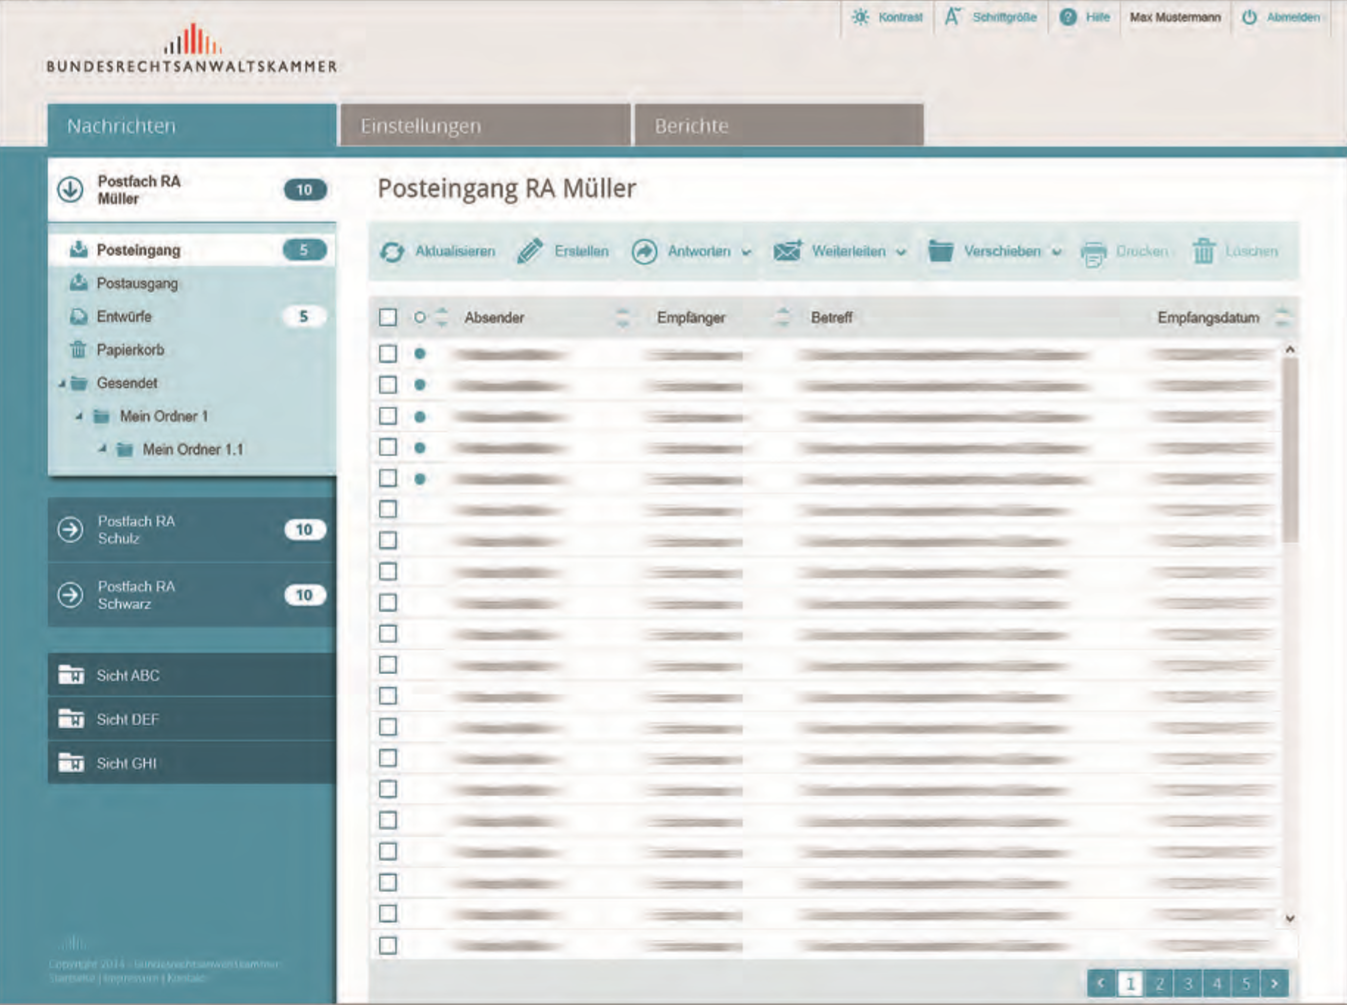
\includegraphics[width=\textwidth]{beA-ui1.png}
	\label{bea:gui:overview}
\end{center}

In Abbildung \ref{bea:gui:overview} ist die vorläufige Oberfläche des beA zu sehen. Man findet die typischen Ordner Posteingang und -ausgang, Entwürfe, Papierkorb und Gesendet vor, auf die der angemeldete Nutzer Zugriff hat. Beim beA kann der jeweilige Rechtsanwalt nur sein eigenes Postfach einsehen. Allerdings kann man Mitarbeitern bestimmte Rechte zuweisen, damit diese beispielsweise den Posteingang sehen und lesen können. Dadurch ist es auch möglich Urlaubsvertretungen festzulegen. Insgesamt wird es mehr als 30 Rechte geben, die man als Postfachinhaber an andere vergeben kann. Darunter fallen Lese-Rechte für bestimmte Ordner, das Recht Nachrichten zu versenden oder sogar das Recht, Rechte an andere vergeben zu dürfen. Durch dieses Rechte-System soll das geforderte jedoch nicht umgesetzte Kanzlei-Postfach simuliert werden. \\
''[...] Einen Wermutstropfen gibt es allerdings: Ein separates Kanzlei- oder Sozietätspostfach wird es nicht geben. Der Gesetzgeber wollte eine eindeutige Adressierbarkeit des einzelnen Rechtsanwaltes gewährleisten und hat daher in der BRAO festgelegt, dass nur Rechtsanwälte ein Anwaltspostfach erhalten. Um hier aber für anwaltliche Organisationseinheiten dennoch ein komfortables Arbeiten zu ermöglichen, gibt es so genannte Sichten (siehe Abbildung \ref{bea:gui:sichten}), die frei definierbar sind. Beispielsweise ist postfachübergreifend die Ansicht aller ungelesenen Nachrichten einstellbar, so dass eine Mitarbeiterin auf einen Blick alle neuen Nachrichten aus allen Postfächern, für die sie zugriffsberechtigt ist, sehen kann. So entsteht faktisch ein ''virtuelles Kanzleieingangspostfach''. Niemand muss sich durch alle Postfächer einzeln durchklicken. [...]''\textcite{bea:bea:brak3/2015} \\
Allerdings können nur Rechte für Personen vergeben werden, die auch im Verzeichnis des beAs zu finden sind, demgemäß zugelassene Rechtsanwälte. In der Realität wird die Post eines Anwalts in Kanzleien meist nicht verwaltet, es gibt Sekretäre oder Sekretärinnen, die sich darum kümmern. Meist handelt es hierbei nicht um zugelassene Rechtsanwälte, weshalb sie auch keinen Zugriff auf das besondere elektronische Anwaltspost haben und damit auch keine Rechte zugewiesen bekommen können. Dies wird sich in der Praxis durch die hohen Sicherheitsvorkehrungen gewiss als hinderlich erweisen.

\subsection{Wie werden Nachrichten versendet?}
Das Versenden einer Nachricht gleicht dem einer E-Mail. Aufgrund der Ende-zu-Ende-Verschlüsselung ist der Nachrichtenbetreff nicht einsehbar, da er auch verschlüsselt wird. Lediglich die Identität des Absenders und das Datum kann man im Klartext lesen. Wurde die Nachricht seitens des Empfängers einmal geöffnet und damit entschlüsselt, ist der Betreff lesbar. Wird sie hiernach geschlossen, wird der Nachrichten-Inhalt inklusive aller Anhänge abermals verschlüsselt, der Betreff bleibt fortan in der Nachrichtenübersicht lesbar. Die Ursache hierfür ist der zweistufige Sicherheitscontainer des Sicherheitsprotokolls OSCI, welches für das Verschlüsseln der Nachrichten verantwortlich ist. Hier werden Inhalts- und Nutzungsdaten streng voneinander getrennt und können dadurch kryptographisch unterschiedlich behandelt werden. Dies ist vor allem für die Datenvermittlung notwendig.\textcite{bea:osci} \footfullcite{bea:osci} Weitere Details über das Sicherheitsprotokoll OSCI sind im Kapitel TODO: zu finden. \\
Nachrichten liegen niemals unverschlüsselt im beA-System vor. Eingegangene Nachrichten können wie bei herkömmlichen E-Mail-Clients nach Belieben sortiert werden, um so schnellsten Zugriff und Übersicht zu erreichen.
Eine weitere wichtige Neuerung ist das elektronische Empfangsbekenntnis. Ab Anfang 2018 wird es dieses als maschinenlesbaren Datensatz geben, der automatisch ausgestellt, zurückgeschickt und anschließend eingelesen werden kann. Bis dahin kann ein Empfangsbekenntnis auf dem normalen Weg - sprich per Post oder Fax, oder qualifiziert elektronisch signiert als Anhang einer beA-Nachricht verschickt werden. 

\begin{figure}[ht]
	\subfigure[Sichten im Postfach]{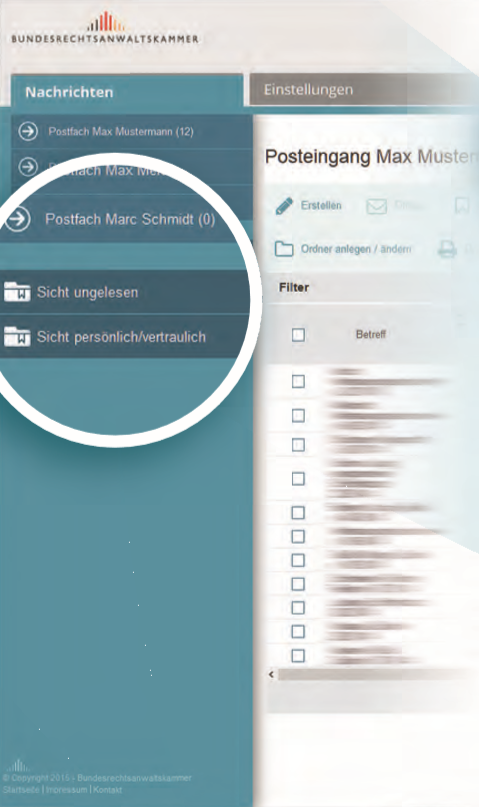
\includegraphics[width=0.49\textwidth]{beA-ui2.png}}
	\subfigure[Postfächer]{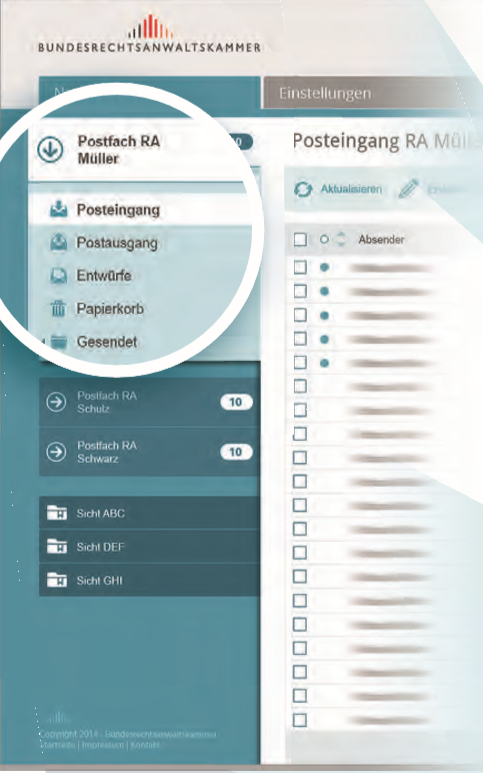
\includegraphics[width=0.49\textwidth]{beA-ui3.png}}
	\caption{Die Navigation innerhalb des Postfachs}
	\label{bea:gui:sichten}
\end{figure}


\subsection{Nachrichten versenden und weiterbearbeiten}
Der Versand der beA-Nachrichten gestaltet sich recht einfach. Es gibt ein Adressverzeichnis, in dem alle Gerichte, Rechtsanwälte, Kammern und sonstigen Empfänger, die über das beA erreicht werden können, aufgelistet sind. Dabei ist zu beachten, dass noch nicht alle Gerichte das beA ab dem 01.01.2015 unterstützen werden. \\
Die Absenderzeile wird vom System automatisch ausgefüllt. Für die maschinelle Verarbeitung und Struktur ist es möglich das eigene und das gerichtliche Aktenzeichen und das der Gegenseite anzugeben. Diese Daten werden beispielsweise als Nutzungsdaten behandelt und dadurch vom OSCI-Standard anders verschlüsselt, als der Nachrichteninhalt. Folglich sind sie - wie bereits im vorigen Kapitel erwähnt, nach dem ersten Entschlüsseln sichtbar. Typischerweise können auch Anhänge zur Nachricht hinzugefügt werden. ''[...] In der Regel wird es sich dabei um Schriftsätze und deren Anlagen handeln. Bezüglich der Nachrichtengröße und der Anzahl der Anhänge orientiert sich das beA an den Vorgaben der Justiz, die voraussichtlich der Hauptadressat von beA-Nachrichten sein wird. Da eine Nachricht gleichzeitig an mehrere Empfänger adressiert werden kann, z.B. an ein Gericht und einen Anwalt, kann für die Kommunikation zwischen Rechtsanwälten nichts anderes gelten. Nach den Vorgaben des Justizstandards dürfen Nachrichten derzeit nicht größer als 30MB sein und nicht mehr als 100 Anhänge umfassen. Die Erweiterung auf 150 MB und 500 Anhänge ist bereits beschlossen. Die verwendbaren Dateiformate richten sich nach den Rechtsverordnungen der Länder, das beA macht hier keine Vorgaben. Einschränkungen wird es nur bei Dateiendungen geben, die eindeutig auf eine Schadsoftware hinweisen. [...]''\textcite{bea:bea:brak3/2015} \\
\\
Eingegangene Nachrichten können - wie bei herkömmlichen E-Mail-Clients, beantwortet oder zu einem anderen beA-Postfach weitergeleitet werden. Zudem kann man Nachrichten ausdrucken oder exportieren. Das beA ist, aufgrund der benötigten Kapazität und damit verbundenen Kosten, kein Nachrichtenarchiv. ''[...] Nachrichten sollten daher nicht im beA belassen werden, sondern in regelmäßigen Abständen in das eigene Dateiablagesystem exportiert oder ausgedruckt und gelöscht werden. Die BRAK wird voraussichtlich innerhalb des ersten Jahres nach Inbetriebnahme des beA-Systems Fristen festlegen, nach deren Ablauf der Postfachinhaber darüber informiert wird, dass Nachrichten automatisch in den Papierkorb verschoben und später dann gelöscht werden. [...]''\textcite{bea:bea:brak3/2015}

\subsection{qualifizierte elektronische Signatur (qeS):}
Bis zum 31.12.2017 müssen Nachrichten, die über das beA verschickt werden, eine qualifizierte elektronische Signatur beinhalten. Das beA wird so konstruiert, dass bis zu diesem Zeitpunkt anderenfalls technisch ein Versand nicht möglich ist. Die Signatur kann dabei der Nachricht selbst oder aber einem Anhang beigefügt werden. Am 1.1.2018 tritt dann der neue § 130a ZPO in Kraft. Danach können auch Dokumente ohne Einsatz der qualifizierten elektronischen Signatur bei Gericht eingereicht werden, wenn sie auf einem sicheren Übermittlungsweg – als solches gilt das beA – eingereicht werden. Das gilt allerdings nur, soweit die Dokumente vom Postfachinhaber selbst – also dem Rechtsanwalt – übersandt werden. Übernimmt ein Mitarbeiter oder eine Mitarbeiterin die Versendung, müssen die Dokumente auch nach dem 1.1.2018 qualifiziert elektronisch signiert werden.

\subsection{Technische Voraussetzungen zur Nutzung}
Der Zugriff auf das beA ist einfach und unkompliziert: Er erfolgt entweder über einen Webbrowser (beispielsweise Firefox, Internetexplorer, Safari oder Chrome) oder direkt aus der Kanzleisoftware heraus. Den Kanzleisoftwareherstellern wird dazu eine entsprechende Schnittstelle zur Verfügung gestellt. Derzeit arbeitet die mit der Entwicklung des beA beauftragte Firma Atos mit Hochdruck an einer solchen Schnittstelle, damit den Kanzleisoftwareherstellern genügend Zeit für die technische Implementierung des beA bleibt.\\
\\
Was wird gebraucht?
\begin{itemize}
\item leistungsfähige Internetverbindung (mind. 2mbit/s)
\item Computer mit mind. 512 MB Arbeitsspeicher und AMD- oder Intel-Prozessor
\item Aktuelles Betriebssystem: Windows, MacOS oder Linux
\item (beA-)Signaturkarte und Kartenlesegerät \textbf{mit Tastatur}
\item Drucker und Scanner
\end{itemize}

\subsubsection{Probleme mit der Internetverbindung}
Da eine Datenrate von 2 Mbit/Sekunde leider noch nicht überall in Deutschland verfügbar ist, wurde der rechtliche Rahmen im ERV-Gesetz so gestaltet, dass bei nachgewiesener Unmöglichkeit einer elektronischen Übersendung zum Gericht auch ein konventioneller Versand möglich sein wird. Dennoch ist dieser Zustand unbefriedigend: Die BRAK wird sich deshalb auf allen politischen Kanälen für einen zügigen Ausbau des Breitbandnetzes einsetzen. Immerhin haben die Regierungsfraktionen in ihrer Koalitionsvereinbarung von 2013 versprochen, dass es bis 2018 in Deutschland eine flächendeckende Grundversorgung mit mindestens 50 Mbit/Sekunde geben soll.

\subsubsection{Kartenlesegeräte}
Die Anmeldung im beA wird voraussichtlich über eine Sicherheitskarte und eine PIN erfolgen. Da insbesondere die Erstanmeldung höchst sicherheitssensibel ist, wird derzeit darüber nachgedacht, dafür eine eigene beA-Karte herauszugeben. Die näheren Fragen dazu – beispielsweise, wo die Karte erhältlich ist oder welche zusätzlichen Eigenschaften (z.B. Signierfunktion) sie hat – werden in den kommenden Wochen geklärt. Angesichts dieser Planungen wird jedoch vom vorsorglichen Erwerb einer der derzeit erhältlichen Signaturkarten abgeraten. Aktuelle Informationen finden Sie jeweils auf der Seite www.bea.brak.de. Es muss ein Kartenlesegerät verwendet werden, das in Deutschland für die Erzeugung einer qualifizierten elektronischen Signatur (qeS) zugelassen ist, denn bis 2018 müssen über das beA versendete Dokumente auf diese Weise signiert werden. Das Kartenlesegerät muss mit einem Tastaturblock, dem sogenannten PIN-Pad ausgestattet sein, dadurch ist es möglich, eine PIN unabhängig von der Computertastatur einzugeben. Das Kartenlesegerät wird über einen USB-Anschluss an den Computer angeschlossen, die digitale Verbindung erfolgt über eine Treibersoftware, die vom Hersteller des Kartelesegerätes mitgeliefert wird und vom Benutzer zu installieren ist. Der Zugang für Mitarbeiter oder sonstige zum Zugriff auf das jeweilige Postfach befugte Personen ist auch möglich über ein sogenanntes Softwarezertifikat, das auf einem Speichermedium, das heißt auf einem USB-Stick, einer Karte o. ä., oder auf dem zu benutzenden Rechner direkt gespeichert ist. Ein solches Softwarezertifikat kann jedoch nicht zur Erstellung einer qualifizierten elektronischen Signatur verwendet werden. Wird das Softwarezertifikat direkt auf dem Rechner gespeichert, sind weitere Sicherheitsvorkehrungen notwendig, so dass sich wegen des geringeren technischen Aufwandes auch für diesen Personenkreis die Verwendung einer Sicherheitskarte – dann ohne Signierfunktion – empfiehlt.

\subsubsection{Drucker und Scanner}
Um das beA effektiv in der Kanzlei einzusetzen, ist in der Regel ein Drucker, ein Scanner oder eine Kombination aus beiden erforderlich. Der Scanner sollte auf verschiedene Auflösungen einstellbar sein, so dass die Pixeldichte je nach Dokumententyp – Textdatei oder Bilddatei – individuell einstellbar ist. Eine geringere Auflösung bedeutet eine geringere Dateigröße und damit einen einfacheren Versand der Nachrichtenanhänge.

\subsubsection{beA-Nutzung in der Kanzlei}
\textit{Das beA wird sich in die grundsätzlichen Arbeitsabläufe und die Arbeitsteilung in der Kanzlei einfügen: Mitarbeitern und Kollegen können verschiedene Zugriffs- und Bearbeitungsrechte eingeräumt werden, sodass die Post auch durch entsprechend ermächtigte Dritte bearbeitet werden kann. Für Kanzleien mit mehreren Berufsträgern ist es durch die Vergabe von Zugriffsrechten möglich, faktisch ein "virtuelles Kanzleipostfach" einzurichten, das die Postein- und -ausgänge mehrerer oder aller Rechtsanwälte der Kanzlei enthält.} \\
\\
Sicher bedeuten diese Anschaffungen zunächst einmal einen gewissen finanziellen Aufwand für jede Kanzlei. Dem gegenüber stehen jedoch deutliche Ersparnisse bei den Papier- und Portokosten und vor allem auch langfristig Vereinfachungen in den alltäglichen Arbeitsabläufen. Dabei fügt sich das beA selbstverständlich umso besser in den Arbeitsalltag ein, je stärker die Kanzlei an sich digitalisiert ist. Auch wenn die Nutzung des beA eine elektronische Aktenführung nicht voraussetzt, bietet die Einführung doch eine gute Gelegenheit auch insgesamt über eine Digitalisierung der Kanzlei nachzudenken.

\subsection{Sicherheitstechnische Mittel}
\begin{itemize}
\item Ende-zu-Ende-Verschlüsselung
\begin{itemize}
\item gewährleistet Vertraulichkeit und Integrität
\item Daten werden beim Sender verschlüsselt und erst beim Empfänger entschlüsselt
\item Dadurch sollen keine anderen Partien während der Übertragung den Inhalt im Klartext lesen können.
\item Gg. Man-in-the-Middle-Attacks generieren beide Enden einen eigenen StringIdentifier basierend auf den PublicKeys der Partien. Diese Identifier werden untereinander Partien ausgetauscht, so dass beide Enden prüfen können, ob ein Man-in-the-Middle sitzt.
\item Verwundbare Punkte: beide Enden. Es muss sichergestellt werden, dass der eigene Computer nicht korrumpiert wurde: denn so könnte der PrivateKey geklaut werden.
\item Die zu übermittelnden Daten werden mit einer sog. Ende-zu-Ende-Verschlüsselung abgesichert, sodass während der Übertragung Dritte (auch Administratoren oder die BRAK selbst) keine Einsichts- und Zugriffsmöglichkeiten auf Nachrichteninhalte haben.
\end{itemize}
\item Sicherheitskarte, Kartenleser und PIN
\begin{itemize}
\item Kartenlesegerät inkl. PIN, um Karte benutzen zu können
\item Spezielle Kryptographie-Software, die die Karte benutzt, um Dokumente elektronisch zu signieren.
\item Hierzu wird ein paar von Schlüsseln benutzt, die verschieden sind, sich aber eindeutig einander zuordnen lassen. Dabei handelt es sich um einen privaten Schlüssel (Signaturschlüssel) und einen öffentlichen Schlüssel (Signaturprüfschlüssel). Der private Schlüssel bleibt geheim, während der öffentliche Schlüssel jedem zugänglich ist (öffentlicher Schlüssel muss vom Hersteller zertifiziert sein!).
\item Ein Dokument, welches vom privaten Schlüssel signiert wurde, kann nur mit dem öffentlichen Schlüssel überprüft werden. Dadurch kann der Absender einer signierten Nachricht immer eindeutig festgestellt werden.
\item Ein weiteres Merkmal: wird der Inhalt unterwegs verändert, ändert sich damit auch die Prüfsumme der Nachricht und der Signaturprüfschlüssel schlägt fehl.
\item Damit bietet dieses Verfahren Authentizität und Integrität.
\end{itemize}
\end{itemize}

\subsubsection{Technische Grundlage: S.A.F.E.-Domäne}
Der ERV wird in einer technisch neuen Infrastruktur mit Einsatz einer Service Oriented Architecture errichtet. Als Grundlage dienen eine S.A.F.E. Domäne, Kommunikationsplattformen und Referenzarchitekturen für die SOA-Dienste \\

Das ERV-Gesetz sieht zudem vor, dass das Postfach im bundesweiten Anwaltsverzeichnis eingerichtet wird, § 31a Abs. 1 BRAO n.F. wodurch sichergestellt ist, dass nur zugelassene Anwälte mit den Gerichten elektronisch kommunizieren können. Diese vertrauen im Sinne des bundesweit anerkannten Konzepts „Secure Access To Federated E-Justice“ (S.A.F.E.) auf die Richtigkeit des Verzeichnisdienstes der Bundesrechtsanwaltskammer. \\

\noindent
\textbf{S.A.F.E. - Grundkonzeption:}
\begin{itemize}
\item S.A.F.E - Secure Access to Federated eJustice/E-Government - stellt Anwendungen sichere elektronische Identitäten (eIDs) für Personen und Organisationen zur Verfügung. 
\item SAFE ermöglicht die Föderierung via Trust-Domains für die eIDs (Einmal registriert - immer akzeptiert) 
\item Die Kommunikation der Trust-Domains untereinander sowie die Kommunikation zwischen SAFE und den Fachanwendungen erfolgt über Schnittstellen entsprechend offener Standards (z.B. SAML-Token=Schnittstellen zur Abfrage der eIDs und deren Berechtigungen).
\item Grundsätzlich eine eID je Nutzer für alle Anwendungen
\item spezielle Attribute für den OSCI-gestützten elektronischen Rechtsverkehr
\begin{itemize}
\item ein Verschlüsselungszertifikat
\item URL des OSCI-Managers
\item Zertifikat des OSCI-Managers
\end{itemize}
\end{itemize}
\textbf{kurz: App-Server mit mehreren Anwendungen, alle Apps benutzen die gleiche UserDB, User benutzen den gleichen AuthServer}

\subsubsection{Protokollstandard}
Begleitet werden die elektronisch zu übermittelnden Dokumente von maschinenlesbaren Strukturdaten – insbes. die Namen der Beteiligten und das Aktenzeichen -, die es den Gerichten ermöglichen, den übersandten Vorgang automatisiert einer elektronischen Gerichtsakte zuzuordnen. Im Gegenzug fordert die Anwaltschaft, dass auch ihr seitens der Gerichte elektronische Strukturdaten zur Weiterverarbeitung in der Fachsoftware zur Verfügung gestellt werden. Eine solche gleichberechtigte Kommunikation haben die Bundesländer zugesagt.\\
OSCI=Online Services Computer Interface:\\
OSCI-Transport ist ein Protokollstandard zur vertraulichen und sicheren Übermittlung von Nachrichten in einer auf das deutsche Signaturgesetz abgestimmten Sicherheitsumgebung
\begin{itemize}
\item Name eines Protokollstandards für die deutsche öffentliche Verwaltung
\item Er steht für mehrere Protokolle, deren gemeinsames Merkmal die besondere Eignung für das E-Government ist:
\begin{itemize}
\item OSCI-Transport für die sichere, vertrauliche und rechtsverbindliche Übertragung digitaler Daten über das Internet sowie
\item eine Reihe verschiedener Protokolle (OSCI-XÖV-Standards) für den Austausch fachlicher Inhaltsdaten auf XML-Basis zwischen Kunden und Behörden bzw. Behörden untereinander.
\end{itemize}
\end{itemize}

\noindent
OSCI-Transport-Nachrichten haben einen zweistufigen „Sicherheitscontainer“. Dadurch ist es möglich, Inhalts- und Nutzungsdaten streng voneinander zu trennen und kryptografisch unterschiedlich zu behandeln. Die Inhaltsdaten werden vom Autor einer OSCI-Transport-Nachricht so verschlüsselt, dass nur der berechtigte Leser sie dechiffrieren kann. Die Nutzungsdaten werden vom Intermediär für die Zwecke der Nachrichtenvermittlung und die Erbringung der Mehrwertdienste benötigt, sie werden deshalb für denIntermediär verschlüsselt. Der Intermediär kann aber nicht auf die Inhaltsdaten zugreifen. Oft wird hier vom „Prinzip des Doppelten Umschlages“ gesprochen: Die verschlüsselten Inhaltsdaten sind wiederum in einen verschlüsselten Container eingebettet. Ein Angreifer kann wegen dieser Verschlüsselungen weder die Nutzungs- noch die Inhaltsdaten abhören.
Jeder Sicherheitscontainer (für Nutzdaten und Inhaltsdaten) erlaubt die digitale Signatur und die Verschlüsselung des jeweiligen Inhalts. Dadurch sind Vertraulichkeit, Integrität und Authentizität der Nachrichten gewährleistet.
Die Public-Key-Infrastruktur (PKI) innerhalb der OSCI-Kommunikationspartner ist – zumindest für natürliche Personen – in der Regel durch das deutsche Signaturgesetz definiert. Es gibt somit keine geschlossene Anwendergruppe. Der Besitz einer Signaturkarte mit einem qualifizierten Signaturzertifikat nach dem Signaturgesetz und einem Verschlüsselungszertifikat sind für die OSCI-Kommunikation ausreichend. Je nach Sicherheitsanforderung kann auch der Einsatz fortgeschrittener elektronischer Signaturen (ohne Chipkarte) sinnvoll sein, auch dies wird durch OSCI-Transport unterstützt.

\subsubsection{Besondere Sicherheit bei Erstanmeldung}
Derzeit laufen parallel zur technischen Entwicklung die ersten internen Tests des beA-Systems. In den kommenden Monaten werden die Tests mit der Justiz durchgeführt. Im Herbst wird dann der so genannte Rollout durchgeführt, damit – wie gesetzlich vorgesehen – pünktlich ab 1.1.2016 alle Postfächer betriebsbereit sind. Jeder Rechtsanwalt muss sich, bevor er mit dem beA arbeiten kann, einmalig an seinem Postfach registrieren. Da diese so genannte Erstregistrierung besonders sicherheitssensibel ist, wird dafür eine besondere beA-Karte erforderlich sein, die auch die Postfach-Nummer, die sogenannte Safe-ID enthält. Nur mit dieser beA-Karte ist sichergestellt, dass die Inbesitznahme eines beA-Postfaches nicht korrumpierbar ist. Ab wann und wo die beA-Karte erhältlich sein wird, wird derzeit geklärt, aktuelle Informationen dazu unter www.bea.brak.de. Nach der Inbesitznahme kann diese beA-Karte auch zur täglichen Anmeldung im Postfach genutzt werden. Je nach individuellem Bedarf wird sie mit oder ohne Signierfunktion erhältlich sein.

\section{Das beA in der Praxis}
Anwälte erhalten künftig keine herkömmliche E-Mail-Adresse, sondern ihre Adressdaten liegen in einer Datenbank. Nachrichten werden also konkret an den jeweiligen Rechtsanwalt oder das jeweilige Gericht geschickt.
Der Begriff des Anwaltspostfachs ist dabei irritierend. Das Postfach wird keineswegs ein öffentliches sein, sondern nur die Adresse innerhalb des Systems (ist öffentlich). Außerhalb dessen ist über beA keine Kommunikation möglich. Anwälte können also über das Anwaltspostfach keine Mails an Mandanten verschicken, sondern es dient \textbf{ausschließlich der Kommunikation mit Gerichten, Behörden und untereinander}.

\subsection{Kosten für Anwälte}
Die Kosten für die Einrichtung der besonderen elektronischen Anwaltspostfächer werden im Ergebnis von der Anwaltschaft zu tragen sein, da die vom Gesetzgeber zur Einrichtung verpflichtete BRAK diese Kosten auf die regionalen Kammern umlegt, welche diese in Form von Beitragserhöhungen an ihre Mitglieder weiterreicht. \\
Hintergrund: Der Gesetzgeber sieht vor, dass für jeden Anwalt ein Postfach einzurichten ist, da auch jeder Anwalt eine Kanzlei zu unterhalten hat, an die wirksame Zustellungen erfolgen müssen. Die Bundesrechtsanwaltskammer hat den gesetzlichen Auftrag erhalten, die elektronischen Anwaltspostfächer zu errichten und der Anwaltschaft bis zum 1.1.2016 zur Verfügung zu stellen. Die Konzeption, Durch- und Einführung des Projekts beA  wird mit einigem Kostenaufwand verbunden sein, welcher zunächst bei der federführenden Bundesrechtsanwaltskammer entsteht. Dabei werden die initialen Kosten für die Einrichtung der Postfächer naturgemäß höher sein als für deren dauerhafte Unterhaltung. \\
Die für Installation und Einrichtung der besonderen elektronischen Anwaltspostfächer anfallenden Kosten wird die Bundesrechtsanwaltskammer (indirekt) über zusätzliche Beiträge refinanzieren, die ab 2015 von allen Regionalkammern aufzubringen sind. Folglich ist ab 2015 mit  – z.T. erheblich – höheren Kammerbeiträgen (die Rede ist von bis zu 50\% in München) zu rechnen.
Pro Anwalt werden nach neusten Stand voraussichtlich eine Umlage von \EUR{67,00} beanstandet.

\subsection{Kosten für die Kanzleien}
Umbau der internen Architekturen/Systeme, neue Software um mit Schnittstelle des beA zu kommunizieren. keine Kanzleipostfächer stattdessen virtuelle Kanzleipostfächer. Einrichten/Verwaltung dauert, Nutzer müssen können da auch kaputt machen. Wie einfach wird die Verwaltung des Postfachs und der Rechte?? \\
Umdenken müssen Kanzleien mit mehreren Berufsträgern. Nicht mehr die Kanzlei ist die Empfängerin von Nachrichten, sondern der jeweilige Anwalt. "Zwar wird es die Möglichkeit geben, Mitarbeitern sowie Kolleginnen und Kollegen Rechte im Postfach einzuräumen", sagt BRAK-Geschäftsführerin Lummel. Dennoch muss das notgedrungen zu neuen Organisationsstrukturen in den Kanzleien führen. "Gerade Großkanzleien müssen nun darüber nachdenken, wie sie interne Prozesse in Zukunft handhaben wollen", sagt der Software-Industrieverbands-Vorsitzende Bertram. \\
Warum ist ein Postfach nicht kanzlei- sondern personengebunden??? Wer immer das verursacht hat, ignoriert den Umstand, dass es (1) anwaltliche Berufsausübungsgemeinschaften (vulg. Sozietäten) gibt, und dass (2) in diesen Fällen nicht der Anwalt, sondern die Sozietät mandatiert ist. Diese Postfachstruktur stellt Sozietäten vor erhebliche Herausforderungen, aber das ist offenbar nicht so wichtig.
\subsubsection{Vorteile für Kanzleien}
\begin{itemize}
\item Sicherer Datenaustausch und Zustellungsnachweis: Ein wesentlicher Vorteil wird der schnelle und sichere Datenaustausch mit Zustellungsnachweis sein. Über eine Eingangsbestätigung weiß der Anwalt schnell, ob und wann ein Dokument vollständig bei Gericht eingegangen ist (§ 130a Abs. 5 S. 2 ZPO n.F.). Zudem können strukturierte Datensätze elektronisch mit den Gerichten ausgetauscht werden. Bei Einreichung einer Klage wird über das Portal oder die Kanzleisoftware bereits ein eigener Datensatz angelegt, der beispielsweise die Parteidaten enthält. Die Gerichtsverwaltung kann diesen Datensatz in die eigene EDV automatisiert einlesen. Umgekehrt werden die Gerichte die strukturierten Daten auch an die Kanzleien übermitteln, die diese wiederum in ihre Kanzleisoftware einlesen können. Fristen könnten bspw. gleich automatisiert in den Kanzleikalender eingetragen werden und müssen anschließend nur noch durch den sachbearbeitenden Anwalt überprüft werden.
\item Flexibilität und Zeitgewinn: Weiterer Vorteil des elektronischen Rechtsverkehrs ist, dass Arbeitsabläufe innerhalb der Kanzlei straffer und effektiver gestaltet werden können. Die ausschließlich elektronische Arbeit mit PC, Laptop oder Tablet in einem umfassenden E-Workflow kann damit, wenn sie richtig eingesetzt wird, die tägliche Arbeit enorm erleichtern.
\item Die elektronische Aktenführung bietet eine enorme Flexibilität. Denn elektronische Akten sind praktisch von überall, wo ein Netzzugang vorhanden ist, zu erreichen. Auch Akteneinsichten oder Verfahrensstandabfragen werden zukünftig elektronisch und praktisch sogar von zu Hause oder dem Arbeitsplatz aus, möglich werden. Insofern ist ein permanenter und ortsunabhängiger Zugriff möglich. Zukünftig wird der Anwalt oder Rechtssuchende durch den elektronischen Zugang auch nicht mehr an die Öffnungszeiten der Gerichte gebunden sein, sondern hat – ohne Wartezeiten –  zeitlich unbegrenzten Zugriff auf die einzusehenden Dokumente.
\item Effizientere Arbeitsweise und Kostenreduzierung: Eine Kosteneinsparung ergibt sich bereits daraus, dass Portokosten für das Versenden von Schriftsätzen etc. oder für die Anforderung von Akten entfallen – ebenso die Kosten für Versandumschläge und das Ausdrucken oder Kopieren der Akten und Schriftsätze. Außerdem führt eine elektronische Archivierung der Akten dazu, Akten- und Papierberge zu vermeiden. Somit müssen keine zusätzlichen Räumlichkeiten bereitgehalten werden, in denen die Akten aufbewahrt werden. Auch eine umständliche Suche im Aktenkeller entfällt künftig.
\item Eine elektronische Aktenführung ermöglicht zudem eine effektivere Mandatsbearbeitung, als es mit Papierakten möglich ist. Dadurch wird die Aktenbearbeitung effizienter und schneller, denn es steht ein elektronischer Workflow für Sortierung, Suchfunktion und systematische Erfassung von Akteninhalten zur Verfügung. Akteninhalte können dadurch schneller aufgefunden und bearbeitet werden.
\end{itemize}

\subsection{Kommunikation mit dem Mandanten}
Um unabhängig davon mit Mandanten oder Dritten zu kommunizieren, müssen die Advokaten weiterhin eigene Software nutzen – und können hier entscheiden, ob sie verschlüsselt oder unverschlüsselt Mails verschicken wollen. Rechtsanwälte werden also wohl noch lange Zeit verschiedene Systeme parallel laufen lassen müssen.

\subsection{Risiken der Nutzung des ERV}
\begin{itemize}
\item Grundsätzlich ist es möglich, dass das Gericht das elektronische Dokument nicht verarbeiten kann oder dass vorübergehend technische Einrichtungen – z.B. aufgrund von Wartungsarbeiten – nicht verfügbar sind. Für diese Fälle hat der Gesetzgeber aber Vorsorge getroffen. Ist das Dokument nicht zur Bearbeitung geeignet, so teilt das Gericht dies dem Absender mit. Das Dokument gilt zum Zeitpunkt der früheren Einreichung eingegangen, sofern der Absender es unverzüglich in einer für das Gericht geeigneten Form nachreicht und glaubhaft macht, dass es mit dem zuerst eingereichten Dokument inhaltlich übereinstimmt, § 130a Abs. 6 ZPO n.F.
\item Ist die Übermittlung eines elektronischen Dokuments aus technischen Gründen vorübergehend unmöglich, bleibt die Übermittlung nach den allgemeinen Vorschriften zulässig. Die vorübergehende Unmöglichkeit ist bei der Ersatzeinreichung oder unverzüglich danach glaubhaft zu machen, § 130d Satz 2 ZPO n.F.
\item Was passiert bei Übermittlungs- oder Verarbeitungsproblemen (z.B. Server- oder Internetausfall)? Ist die Übermittlung eines elektronischen Dokuments aus technischen Gründen nicht möglich, bleibt selbstverständlich die herkömmliche Übermittlung nach den allgemeinen Vorschriften, d.h. also per Post oder Fax zulässig (§ 130d S. 2 ZPO n. F.).
\end{itemize}

\subsection{Empfangsbekenntnis}
Was wird aus dem bislang üblichen schriftlichen Empfangsbekenntnis (EB) als Zustellungsnachweis (§ 174 Abs. 1 ZPO) bei Zustellungen an den Anwalt? \\
Das bisherige EB wird durch ein elektronisches EB ersetzt (§ 174 Abs. 4 ZPO-neu). Während der Regierungsentwurf ursprünglich eine Abschaffung des schriftlichen Empfangsbekenntnisses vorsah und dieses durch eine vom zukünftig einzurichtenden elektronischen Postfach der Anwälte automatisch erstellte Eingangsbestätigung (nach 3 Tagen) ersetzt werden sollte, wurde im Laufe des Gesetzgebungsverfahrens auf die Kritik der Anwaltsverbände reagiert. Nunmehr ist ein elektronisches Empfangsbekenntnis als Ersatz für das bisherige Empfangsbekenntnis vorgesehen, welches als strukturierter maschinenlesbarer Datensatz zu übermitteln ist.

\subsection{ERV hat auch im Handelsregister geklappt. Wieso?}
\begin{itemize}
\item Kommunikation mit Handelsregister nur noch elektronisch zugelassen seit 2007
\item Maschinell lesbare Antragstellung für automatisiertes Mahnverfahren für Anwälte seit 2008 verpflichtend.
\item Schluss: man macht einfach alles in allen Bereichen verpflichtend $\Rightarrow$ höhere Nutzrate
\item macht nur Sinn, wenn Aufnahme dieser Dokumente und Infrastruktur (Schaffung einer solchen) gegeben sind $\Rightarrow$ Arbeitsgruppe die herausfinden soll, was sich für Gerichte ändert. 
\item Arbeitsgruppe: Umstellung auf ERV wird erwartet von Gesellschaft. Wandel der Gesellschaft: Bürgernähe+moderne Justiz
\item Aktuell: An Pilotgerichten festgestellt: ERV setzt sich nicht durch, weiterhin werden ERV und Papier benutzt $\Rightarrow$ Mehraufwand+Kosten. Was Sinn macht: 
\item Änderungen am geltenden Signaturrecht für wirtschaftlich sinnvolle Umsetzung notwendig.
\item Kosten werden sich kurz/mittelfristig NICHT amotisieren = ERV macht sich kurz/mittelfristig nicht bezahlt. Wirtschaftliche Effekte erst, wenn Ablauf vollständig elektronisiert und Ausbau überall abgeschlossen.
\end{itemize}

\subsection{Schutzschriftenregister}
\textit{Schutzschriften sind vorbeugende Verteidigungsschriftsätze gegen erwartete Anträge auf Arrest oder einstweilige Verfügung. Mit ihnen will der mögliche Antragsgegner erreichen, dass der Antrag zurückgewiesen wird, wenigstens aber verhindern, dass dem Antrag ohne mündliche Verhandlung entsprochen wird. Derzeit muss eine Schutzschrift bei jedem Gericht eingereicht werden, bei dem ein Antrag auf Arrest oder einstweilige Verfügung zu erwarten ist. Die Einreichung einer Schutzschrift bei einem Gericht hat nur Wirkung für dieses Gericht. Sind potentiell mehrere Gerichte zuständig, kann die Einreichung der Schutzschriften einen erheblichen Arbeits- und Sachaufwand bei Antragsgegnern und Rechtsanwälten, aber auch bei den Gerichten verursachen. } \\\\

Es wird ein zentrales, bundesweites elektronisches Schutzschriftenregister eingerichtet, bei dem die Einreichung einer Schutzschrift genügt, um alle Zivil- und Arbeitsgerichte zu erreichen. § 945a Absatz 2 Satz 1 der Zivilprozessordnung (ZPO) sowie § 62 Absatz 2 Satz 3 und § 85 Absatz 2 Satz 3 des Arbeitsgerichtsgesetzes (ArbGG), jeweils in der zum 1. Januar 2016 in Kraft tretenden Fassung des Gesetzes zur Förderung des elektronischen Rechtsverkehrs mit den Gerichten vom 10. Oktober 2013 (BGBl. I S. 3786), sehen deshalb vor, dass eine bei dem Register eingereichte Schutzschrift als bei allen Zivil- und Arbeitsgerichten der Länder eingereicht gilt. Die zentral hinterlegten Schutzschriften können von den Gerichten elektronisch abgerufen werden (§ 945a Absatz 3 Satz 1 ZPO). Die näheren Bestimmungen über die Einrichtung und Führung des Registers, über die Einreichung von Schutzschriften zum Register, über den Abruf von Schutzschriften aus dem Register sowie über die Einzelheiten der Datenübermittlung und -speicherung sowie der Datensicherheit und der Barrierefreiheit werden auf Grundlage des § 945b ZPO durch Verordnung geregelt.\\\\

\textbf{Für Rechtsanwälte wird das Elektronische Schutzschriftenregister über das beA erreichbar sein.}

\section{Besonderes elektronisches Notarpostfach}
Notare nutzen das besondere Notarpostfach, dessen Bereitstellung im Verantwortungsbereich der Bundesnotarkammer liegt. So werden alle Notare im Zuge des Updates der Fachsoftware XNotar auf Version 3.5.x mit einem EGVP-Programm ausgestattet. Die NotarNet GmbH wird rechtzeitig auf alle Lizenzinhaber zukommen.

Kommt mit dem beA!!! Genau das gleiche nur für Notare….
Notare haben bisher ein Notarpostfach im EGVP gehabt, siehe Gieselmann-Elektronischer-Rechstverkehr-mit-dem-Handelsregister.pdf.